\documentclass[a4paper, 12pt]{article}%тип документа

%отступы
\usepackage[left=2cm,right=2cm,top=2cm,bottom=3cm,bindingoffset=0cm]{geometry}

%Русский язык
\usepackage[T2A]{fontenc} %кодировка
\usepackage[utf8]{inputenc} %кодировка исходного кода
\usepackage[english,russian]{babel} %локализация и переносы

%Вставка картинок
\usepackage{wrapfig}
\usepackage{graphicx}
\usepackage{subcaption,floatrow}
\graphicspath{{images/}}
\DeclareGraphicsExtensions{.pdf,.png,.jpg}

\DeclareFloatSeparators{mysep}{\hspace{1cm}}

%оглавление
\usepackage{titlesec}
\titlespacing{\chapter}{0pt}{-30pt}{12pt}
\titlespacing{\section}{\parindent}{5mm}{5mm}
\titlespacing{\subsection}{\parindent}{5mm}{5mm}
\usepackage{setspace}

%Графики
\usepackage{multirow}
\usepackage{pgfplots}
\pgfplotsset{compat=1.9}

%Математика
\usepackage{amsmath, amsfonts, amssymb, amsthm, mathtools}

%Стиль страницы
\usepackage{fancyhdr}
\pagestyle{fancy}

\begin{document}

\begin{titlepage}

\begin{center}
%\vspace*{1cm}
\large\textbf{Московский Физико-Технический Институт}\\
\large\textbf{(государственный университет)}
\vfill
\line(1,0){430}\\[1mm]
\huge\textbf{Работа 5.1.2}\\
\line(1,0){430}\\[1mm]
\vfill
\large Сибгатуллин Булат, ФРКТ\\
\end{center}

\end{titlepage}
\fancyhead[L] {Работа 5.1.2}
\noindent \textbf{Цель работы: } \\
\indent с помощью сцинтиляционного спектрометра исследуется энергетический спектр $\gamma$-квантов, рассеянных на графите. Опреляется энергия рассеянных $\gamma$-квантов в зависимости от угла рассеяния, а также энергия покоя частиц, на которых происходит комптоновское рассеяние.

\section{Теоретическая часть}
	Эффект Комптона -- увеличение длины волны рассеянного излучения по сравнению с падающим -- интерпретируется как результат упругого содуранеия двух частиц: $\gamma$-кванта и свободного электрона.
	
	Из закона сохранения 4-имульса для системы <<фотон + электрон>> следует формула для изменения длины волны рассеянного излучения:
	\begin{equation}\label{Kompton}
		\Delta \lambda = \Lambda_K(1-\cos\theta),
	\end{equation}
	где величина $\Lambda_K = h/(mc) = 2,42 \cdot 10^{-10}$ см называется комптоновской длиной волны электрона.
	
	Из формулы (\ref{Kompton}) следует, что комптоновское смещение не зависит ни от длины волны первичного излучения, ни от рода вещества, в котором наблюдается рассеяние. В общем случае комптоновоское рассеяние происходит на свободных электронах в атоме. Для $\gamma$-квантов с энергией в несколько десятков, а тем более сотен килоэлектрон-вольт, связь электронов в атоме мало существенна, так как энергрия их связи в легких атомах не превосходит нескольких килоэлектрон-вольт, а для большинства электронов еще меньше.
	
	При рассеянии на связанных электронах изменение импульса кванта воспринимается атомом в целом. Посколько масса атома очень велика, переда ча импульса не спровождается сколь-нибудь заметной передачей энергии, и наблюдается несмещенная (по энергии) компонента в спектре рассеянного излучения. Таким образом, рассеяние $\gamma$-квантов на связанных электронах можно рассматривать как упругое столкновение квантов с атомами.
	
	Основной целью данной работы является проверка соотношения (\ref{Kompton}). Применительно к условиям нашего опыта формулу (\ref{Kompton}) следует преобразовать от длин волн к энергиям $\gamma$-квантов. Как нетрудно показать, соответсвующиее выражение имеет вид:
	\begin{equation}\label{1-cos}
		\frac{1}{\varepsilon(\theta)} - \frac{1}{\varepsilon_0} = 1 - \cos \theta.
	\end{equation}

	Здесь $\varepsilon_0 = E_0/(mc^2)$ -- выраженная в единицах $(mc^2)$ энергия $\gamma$-квантов, падающих на рассеиватель, $\varepsilon(\theta)$ -- выраженная в тех же единицах энергия квантов, испытавших комптоновское рассеяние на угол $\theta$, $m$ -- масса электрона.
	
	Заменим в формуле~(\ref{1-cos}) энергию квантов, испытавших комптоновское рассеяние на угол $\theta$, номером канала $N(\theta)$, соответствующего вершине фотопика при указанном угле $\theta$:
	\begin{equation}\label{kek}
		\frac{1}{N(\theta)} - \frac{1}{N(0)} = A (1- \cos \theta),
	\end{equation}
	где $A$ -- неизвестный коэффциицент пропорциональности между $\varepsilon(\theta)$ и $N(\theta)$.
\newpage
\section{Экспериментальная установка}
	Блок-схема установки изображена на рис.~\ref{pic1}. Источником излучения 1 служит $^{137}$Cs, испускающий $\gamma$-лучи с энергией 662 кэВ. Он помещен в толстенный свинцовый контейнер с коллиматором. Сформмированный коллиматором узкий пучок $\gamma$-квантов попадает на графитовую мишень 2 (цилиндр диамтером 40 мм и высотой 100 мм.)
	
	
	\thisfloatsetup{floatrowsep=mysep}	
	\begin{figure}[h!]
		\ffigbox{
			\begin{subfloatrow}[2]
				\ffigbox[\FBwidth]{\caption{}}%
				{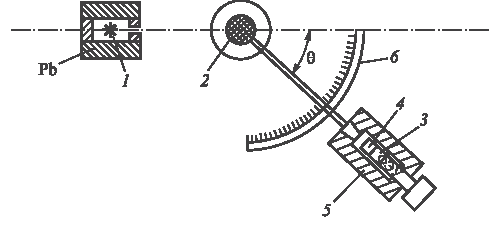
\includegraphics[scale=1]{images/ustanovka1.pdf}{\label{pic1}}}
				\ffigbox[\FBwidth]{\caption{}}%
				{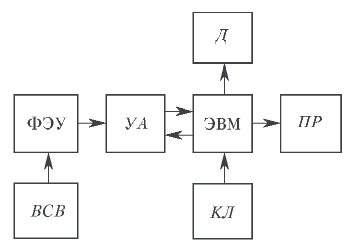
\includegraphics[scale=1]{images/ustanovka2.pdf}{\label{pic2}}}         
			\end{subfloatrow}
		}
		{\caption{Экспериментальная установка.}}
	\end{figure}
	
	Кванты, испытавшие комптоновское рассеяние в мишени, региструруются сцинтилляционным счетчиком. Счетчик состоит из фотоэлектронного умножителя 3 (далее ФЭУ) и сцинтиллятора 4. Сцинтиллятором служит кристалл NaI(Tl) цилиндрической формы диаметром 40 мм и высотой 40 мм, его выходное окно находится в оптическом контакте с фотокатодом ФЭУ. Сигналы, возникающие на ФЭУ, подаются на ЭВМ для амплитудного анализа. Кристалл и ФЭУ расположены в светонепроницаемом блоке, укрепленном на горизонтальной штанге. Штанга вместе с этим блоком может вращаться относительно мишени, угол поворота отсчитывается по лимбу 6.
	
	На рис.~\ref{pic2} представлена функциональная блок-схема измерительного комплекса, который состоит из ФЭУ, питаемого от высоковольтного выпрямителя ВСВ, обеспечивающего работу ФЭУ в спектрометрическом режиме, усилителя-анализатора УА, являющегося входным интерфейсом ЭВМ, управляемой с клавиатуры КЛ. В ходе проведения эксперимента информация отражается на экране дисплея Д, окончательные результаты в виде таблиц и графиков могут быть выведены на принтер ПР.

\section{Ход работы}

\begin{enumerate}
\item Включим все устройства и компьютер. Откроем программу и войдем в режим измерения спектра.

\thisfloatsetup{floatrowsep=mysep}	
	\begin{figure}[h!]
		\ffigbox{
			\begin{subfloatrow}[2]
				\ffigbox[\FBwidth]{\caption{}}%
				{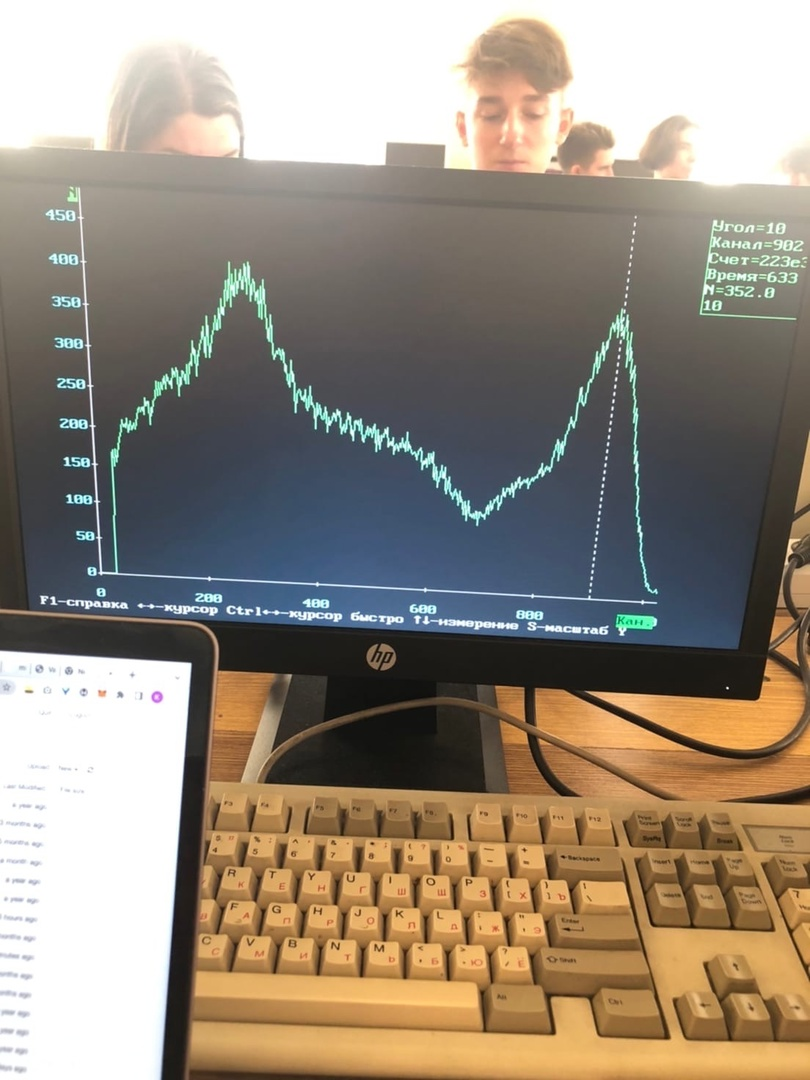
\includegraphics[width = 1\linewidth]{images/10.jpg}{\label{pic1}}}
				\ffigbox[\FBwidth]{\caption{}}%
				{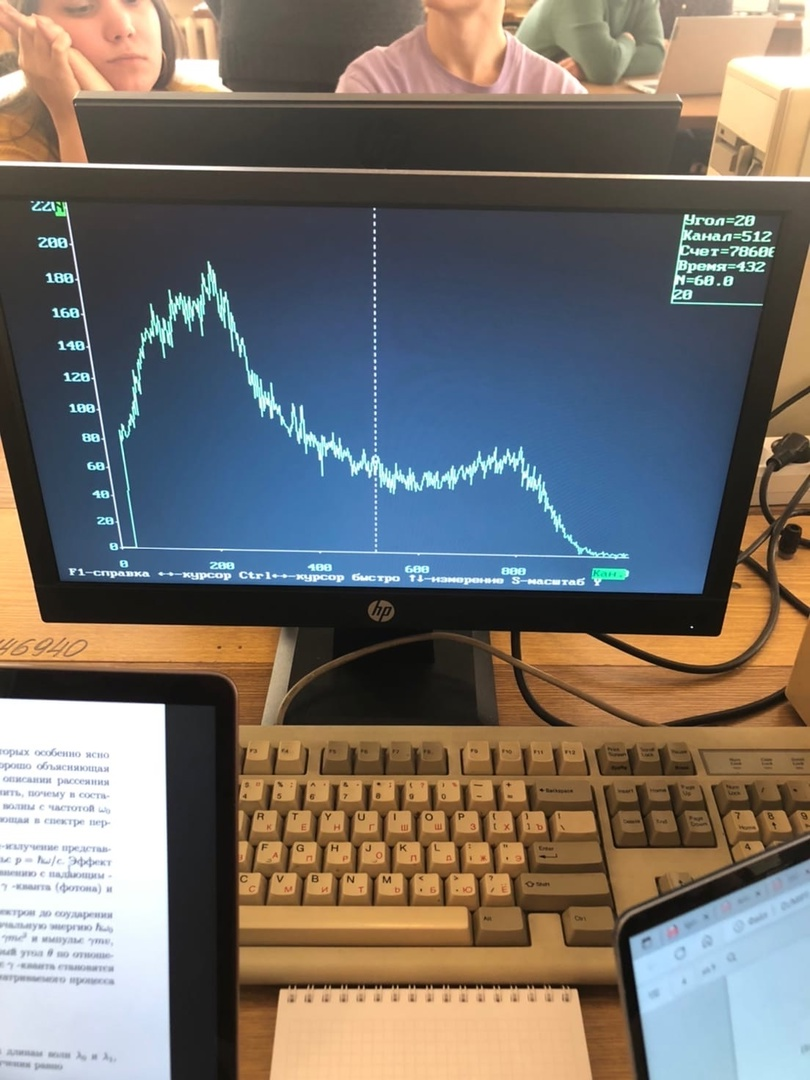
\includegraphics[width = 1\linewidth]{images/20.jpg}{\label{pic2}}}         
			\end{subfloatrow}
		}
		{\caption{Экспериментальная установка.}}
	\end{figure}

\item Снимем амплитудные спектры и определим положения фотопиков для каждого угла $\theta$. Погрешность измерения угла возьмем равной $\sigma_{\theta} = 0,5^{\circ}$, а $N_0$ за $N$ от нуля градусов:

\begin{center}
\begin{tabular}{|c|c|c|c|c|c|c|}
\hline 
$\theta$ & $1 - \cos (\theta )$ & $\sigma_{1 - \cos (\theta )}$ & $N$ & $1/N - 1/N_0$ & $\sigma_N$ & $\sigma_{1/N - 1/N_0}$ \\ 
\hline 
0 & 0 & 0,00002 & 832 & - & 25 & - \\ 
\hline 
10 & 0,0152 & 0,00017 & 902 & -0,00009 & 25 & $4\cdot 10^{-6}$ \\ 
\hline 
20 & 0,0603 & 0,00067 & 766 & 0,00010 & 40 & $8\cdot 10^{-6}$ \\ 
\hline 
30 & 0,1340 & 0,00149 & 717 & 0,00019 & 60 & $1,6\cdot 10^{-5}$ \\ 
\hline 
40 & 0,2340 & 0,00260 & 687 & 0,00025 & 60 & $1,8\cdot 10^{-5}$ \\ 
\hline 
50 & 0,3572 & 0,00397 & 608 & 0,00044 & 50 & $3,6\cdot 10^{-5}$ \\ 
\hline 
60 & 0,5000 & 0,00556 & 512 & 0,00075 & 50 & $7,3\cdot 10^{-5}$ \\ 
\hline 
70 & 0,6580 & 0,00731 & 472 & 0,00091 & 50 & $9,7\cdot 10^{-5}$ \\ 
\hline 
80 & 0,8263 & 0,00918 & 412 & 0,00123 & 50 &0,00015 \\ 
\hline 
90 & 1,0000 & 0,01111 & 392 & 0,00134 & 50 & 0,00017 \\ 
\hline 
100 & 1,1737 & 0,01304 & 345 & 0,00162 & 50 & 0,00025 \\ 
\hline 
110 & 1,3420 & 0,01491 & 309 & 0,00307 & 50 & 0,00033 \\ 
\hline 
\end{tabular} 
\end{center}

\item Построим график зависимости $f(1 - \cos (\theta ))$, где по оси $y$ отложим $1/N - 1/N_0$, а по оси $x$ - $1 - \cos (\theta )$.

\begin{figure}[h!]
\centering
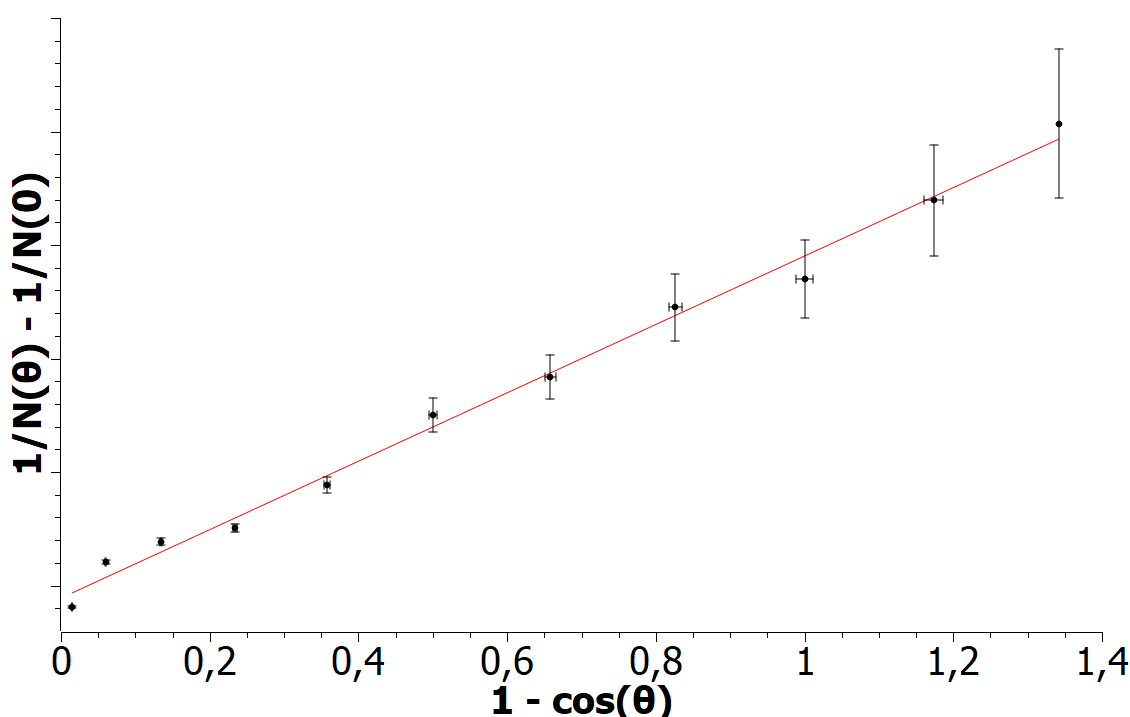
\includegraphics[width = 0.9\linewidth]{images/graph.png}
\caption{График зависимости $1/N - 1/N_0$ от $1 - \cos (\theta )$}
\label{graph}
\end{figure}

Получим линейную зависимость вида $y = ax + b$, с коэффициентами:

\begin{center}
\begin{tabular}{|c|c|c|}
\hline 
 & Значение & Погрешность МНК \\ 
\hline 
a & 0,00151 & 0,00004 \\ 
\hline 
b & $-3,29 \cdot 10^{-5}$ & $2,74 \cdot 10^{-5}$ \\ 
\hline 
\end{tabular} 
\end{center}

Учтем погрешности измерений и получим итоговую погрешность $\sigma_{a res} = 0,00025$.

\item Из формулы \eqref{kek} понимаем, что угловой коэффициент $a$ равен неизвестному коэффициенту $A$. Теперь зная коэффициент $A$ находим, что $mc^2 = 1/A$ при $\theta = 90^{\circ}$. Так как $a$ постоянно при любом значении $\theta$, то и $A$ и $mc^2$ тоже постоянны и не зависят от угла. Следовательно:

\[mc^2 = 662,3 \pm 108,6 \: \text{кэВ}\]

\item По формуле:

\begin{equation}\label{gamma_energy}
mc^2 = E_{\gamma}\frac{N_{best}(90)}{N_{best}(0) - N_{best}(90)}
\end{equation}

Возьмем за $N_{best}(\theta)$ значения $N$ соответствующие измерениям $N$ по МНК для данного угла $\theta$. Тогда $N_{best}(0) = 832$ и $N_{best}(90) = 369$. Здесь погрешность складывается из погрешности $N_{best}(\theta)$ и погрешности $mc^2$.

Получаем:

\[E_{\gamma} = 831 \pm 190 \: \text{кэВ}\]

\end{enumerate}

\section{Вывод}

В данной работе исследоваи эффект Комптона и посмотрели на спектр $\gamma$-квантов рассеяных на графите. Оценили энергию данных $\gamma$-квантов, получили $E_{\gamma} = 831 \pm 190$ кэВ. Табличное значение равно 662 кэВ, поэтому полученное значение сходится с табличным в пределах погрешности. Но при этом погрешность измерения составляет 22,8 $\%$, что является довольно плохим значением. Данная точность обусловлена плохой точностью измерения фотопика (его погрешность вносит основной вклад в это значение). Также мы не учитываем счетную характеристику ФЭУ (колебания напряжения на нем), а она также может вносить погрешность в результаты измерения.

\end{document}